\documentclass[aspectratio=169,c]{beamer} % 16:9 top adjusted

\usepackage[english]{babel}
\usetheme{Darmstadt} % Mertens: Madrid
%\usecolortheme[options]{beamer color theme}

%\setbeamerfont{title}{series=\bfseries, family=\rmfamily}
%\setbeamercolor{title}{fg=white, bg=red!50!black}
%\setbeamertemplate{navigation symbols}{}


\usepackage{tikz}
\usetikzlibrary{snakes,calc}
\usepackage{amsmath}
\usepackage{amssymb}
\usepackage{algorithmic}
\usepackage{algorithm}
\usepackage{ifthen}

%based on https://tex.stackexchange.com/questions/51019/how-can-i-put-a-curly-brace-inside-an-algorithm-to-group-code-lines + chatgpt + own modifications
%\usetikzlibrary{decorations.pathreplacing,calc}
% How to use:
% tikzmark{nodename}
% AddBraceTop{topnode}{bottomnode}{text}{colour}    aligns with x-coord of topnode
% AddBraceBottom{topnode}{bottomnode}{text}{colour} aligns with x-coord of bottomnode
% AddBraceTopShift{topnode}{bottomnode}{text}{colour}{shift} aligns with x-coord of (topnode + shift)
% AddBraceReverseShift{topnode}{bottomnode}{text}{colour}{shift}{textshift}
% AddTextShift{node}{text}{colour}{shift}
% AddArrow{node}{text}{colour}{shift} end of arrow at (node + shift)
\newcommand{\tikzmark}[1]{\tikz[overlay,remember picture] \node (#1) {};}
\newcommand{\AddBraceTop}[4]{%
    \begin{tikzpicture}[overlay, remember picture]
        \draw [decoration={brace,amplitude=0.5em},decorate,ultra thick,#4]
        (#1.north east) --
        (#2.south -| #1.north east) % (#1.x, #2.y)
        node[midway,right=0.5em,align=left,text width=2.5cm] {#3};
    \end{tikzpicture}%
}
\newcommand{\AddBraceTopShift}[5]{%
    \begin{tikzpicture}[overlay, remember picture]
        \draw [decoration={brace,amplitude=0.5em},decorate,ultra thick,#4]
        ($(#1.north east) + #5$) --
        ($(#2.south -| #1.north east) + #5$) % (#1.x, #2.y)
        node[midway,right=0.5em,align=left,text width=2.5cm] {#3};
    \end{tikzpicture}%
}
\newcommand{\AddBraceBottom}[4]{%
    \begin{tikzpicture}[overlay, remember picture]
        \draw [decoration={brace,amplitude=0.5em},decorate,ultra thick,#4]
        (#1.north -| #2.south east) -- % (#2.x, #1.y)
        (#2.south east)
        node[midway,right=0.5em,align=left,text width=2.5cm] {#3};
    \end{tikzpicture}%
}
\newcommand{\AddBraceReverseShift}[6]{%
    \begin{tikzpicture}[overlay, remember picture]
        \draw [decoration={brace,amplitude=0.5em},decorate,ultra thick,#4]
        ($(#2.south -| #1.north west) + #5$) -- % (#1.x, #2.y)
        ($(#1.north west) + #5$)
        node[midway,right=#6,align=left,text width=2.5cm] {#3};
    \end{tikzpicture}%
}
\newcommand{\AddTextShift}[4]{%
    \begin{tikzpicture}[overlay, remember picture]
        \draw ($(#1.north west) + #4$) -- ($(#1.north west) + #4$)
        node[right=0.5em,align=left,text width=2.5cm, #3] {#2};
    \end{tikzpicture}%
}
\newcommand{\AddArrowNorth}[4]{%
    \begin{tikzpicture}[overlay, remember picture]
        \draw [-{stealth},ultra thick,#3]
        ($(#1) + #4$) node[right=0em,align=left,text width=2.5cm] {#2} 
        -- (#1.north);
    \end{tikzpicture}%
}

\title{Flows - secondary slides}
\subtitle{Proseminar Algorithmen auf Graphen}
\author{Nils Wagner}
\institute{RWTH Aachen University}
\date{May 21, 2024}


\begin{document}
\begin{frame}[plain]
    \maketitle
\end{frame}

\begin{frame} % empty slide
\end{frame}

\section{Flow Networks and Maximum-Flow Problem}
\section{Ford-Fulkerson Method}
\begin{frame}{Ford-Fulkerson Method}
    \begin{columns}[c]
        \begin{column}{0.5\textwidth}
            \begin{block}{Ford-Fulkerson Method}
                \begin{algorithmic}[1]
                    \STATE initialize flow \(f\) with 0
                    \WHILE{there exists an augmenting path \(p\) in the residual network \(G_f\)}
                    \STATE augment flow \(f\) along \(p\)
                    \ENDWHILE
                    \RETURN \(f\)
                \end{algorithmic}
            \end{block}
        \end{column}
        \begin{column}{0.5\textwidth}
            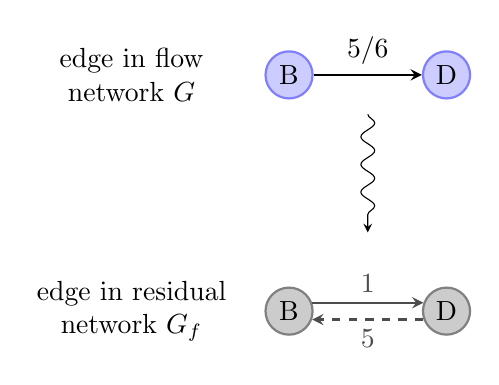
\begin{tikzpicture}
                [%x=10mm, y=9mm, 
                every text node part/.style={align=center},
                nsty/.style={circle, draw=blue!50, fill=blue!20, thick, inner sep=0.15em, minimum size=1.7em},
                gsty/.style={circle, draw=black!50, fill=black!20, thick, inner sep=0.15em, minimum size=1.7em},
                asty/.style={-{stealth}, thick}]
                % flow network
                \node at (0,3) {edge in flow \\network \(G\)};
                \node[nsty] (b) at (2,3) {B};
                \node[nsty] (d) at (4,3) {D};
                \draw[asty] (b) -- node[auto]{5/6} (d);
                % transition
                \draw[-{stealth}, snake=snake, line after snake=1mm] (3,2.5) -- (3,1);
                % residual network
                \node at (0,0) {edge in residual \\network \(G_f\)};
                \node[gsty] (b') at (2,0) {B};
                \node[gsty] (d') at (4,0) {D};
                \draw[asty, black!70] (b'.20) -- node[auto]{1} (d'.160);
                \draw[asty, dashed, black!70] (d'.-160) -- node[auto]{5} (b'.-20);
            \end{tikzpicture}
        \end{column}
    \end{columns}
\end{frame}

\begin{frame}
    \begin{columns}[c]
        \begin{column}{0.86\textwidth}
            \begin{block}{Ford-Fulkerson Method (with DFS)}
                \begin{algorithmic}[1]
                    \FOR{each edge \((u,v)\in E\)\tikzmark{top1}} 
                    \STATE \(f(u,v)\gets 0\)
                    \ENDFOR \tikzmark{bot1}
                    \WHILE{\tikzmark{while0}there exists an augmenting path\tikzmark{path} \(p\) in the residual network \(G_f\)\tikzmark{while}}
                    \STATE \(c_f(p)\gets\min\{c_f(u,v)\mid (u,v)\in p\}\)\tikzmark{top2}
                    \FOR{each edge \((u,v)\in p\)}
                    \IF{\((u,v)\in E\)}
                    \STATE \(f(u,v)\gets f(u,v) + c_f(p)\)
                    \ELSE
                    \STATE \(f(v,u)\gets f(v,u) - c_f(p)\)
                    \ENDIF
                    \ENDFOR \tikzmark{bot2}
                    \ENDWHILE \tikzmark{while1}
                    \RETURN \(f\)
                \end{algorithmic}
            \end{block}
        \end{column}
    \end{columns}
    \AddBraceTop{top2}{bot2}{\(O(E)\)}{red}
    \AddBraceTopShift{top1}{bot1}{\(O(E)\)}{red}{(0.5,0)}
    \AddTextShift{while}{\(O(\lvert f\rvert)\) times}{red}{(0.4,-0.03)}
    \AddArrowNorth{path}{DFS: \(O(E)\)}{red}{(2,1.3)}
    \AddBraceReverseShift{while0}{while1}{\(O(\lvert f\rvert E)\)}{red}{(-1.7,0)}{-1.8cm}
\end{frame}

\begin{frame} % empty slide
\end{frame}

\section{Optimizations of Ford-Fulkerson Method}
\begin{frame}
    \begin{columns}[c]
        \begin{column}{0.86\textwidth}
            \begin{block}{Ford-Fulkerson Method (with BFS) / Edmonds-Karp Algorithm}
                \begin{algorithmic}[1]
                    \FOR{each edge \((u,v)\in E\)\tikzmark{top1}} 
                    \STATE \(f(u,v)\gets 0\)
                    \ENDFOR \tikzmark{bot1}
                    \WHILE{\tikzmark{while0}there exists an augmenting path\tikzmark{path} \(p\) in the residual network \(G_f\)\tikzmark{while}}
                    \STATE \(c_f(p)\gets\min\{c_f(u,v)\mid (u,v)\in p\}\)\tikzmark{top2}
                    \FOR{each edge \((u,v)\in p\)}
                    \IF{\((u,v)\in E\)}
                    \STATE \(f(u,v)\gets f(u,v) + c_f(p)\)
                    \ELSE
                    \STATE \(f(v,u)\gets f(v,u) - c_f(p)\)
                    \ENDIF
                    \ENDFOR \tikzmark{bot2}
                    \ENDWHILE \tikzmark{while1}
                    \RETURN \(f\)
                \end{algorithmic}
            \end{block}
        \end{column}
    \end{columns}
    \AddBraceTop{top2}{bot2}{\(O(E)\)}{blue!80}
    \AddBraceTopShift{top1}{bot1}{\(O(E)\)}{blue!80}{(0.5,0)}
    \AddTextShift{while}{\(\ \ \ O(VE)\)\\\ \ \ times}{red}{(0.4,-0.03)}
    \AddArrowNorth{path}{BFS: \color{blue!80}\(O(E)\)}{red}{(2,1.3)}
    \AddBraceReverseShift{while0}{while1}{\(O(V E^2)\)}{red}{(-1.7,0)}{-1.8cm}
\end{frame}

\section{Summary}

\end{document}
